%\documentclass[9pt,twocolumn,twoside,lineno]{pnas-new}
\documentclass[9pt,twocolumn,twoside]{pnas-new}
% Use the lineno option to display guide line numbers if required.
% Note that the use of elements such as single-column equations
% may affect the guide line number alignment. 

\templatetype{pnasresearcharticle} % Choose template 
% {pnasresearcharticle} = Template for a two-column research article
% {pnasmathematics} = Template for a one-column mathematics article
% {pnasinvited} = Template for a PNAS invited submission

\title{Template for preparing your research report submission to PNAS using Overleaf}

% Use letters for affiliations, numbers to show equal authorship (if applicable) and to indicate the corresponding author
\author[a,c,1]{Author One}
\author[b,1,2]{Author Two} 
\author[a]{Author Three}

\affil[a]{Affiliation One}
\affil[b]{Affiliation Two}
\affil[c]{Affiliation Three}

% Please give the surname of the lead author for the running footer
\leadauthor{Lead author last name} 

% Please add here a significance statement to explain the relevance of your work
\significancestatement{Authors must submit a 120-word maximum statement about the significance of their research paper written at a level understandable to an undergraduate educated scientist outside their field of speciality. The primary goal of the Significance Statement is to explain the relevance of the work in broad context to a broad readership. The Significance Statement appears in the paper itself and is required for all research papers.}

% Please include corresponding author, author contribution and author declaration information
\authorcontributions{Please provide details of author contributions here.}
\authordeclaration{Please declare any conflict of interest here.}
\equalauthors{\textsuperscript{1}A.O.(Author One) and A.T. (Author Two) contributed equally to this work (remove if not applicable).}
\correspondingauthor{\textsuperscript{2}To whom correspondence should be addressed. E-mail: author.two\@email.com}

% Keywords are not mandatory, but authors are strongly encouraged to provide them. If provided, please include two to five keywords, separated by the pipe symbol, e.g:
\keywords{Keyword 1 $|$ Keyword 2 $|$ Keyword 3 $|$ ...} 

\begin{abstract}
Please provide an abstract of no more than 250 words in a single paragraph. Abstracts should explain to the general reader the major contributions of the article. References in the abstract must be cited in full within the abstract itself and cited in the text.
\end{abstract}

\dates{This manuscript was compiled on \today}
\doi{\url{www.pnas.org/cgi/doi/10.1073/pnas.XXXXXXXXXX}}

\begin{document}

% Optional adjustment to line up main text (after abstract) of first page with line numbers, when using both lineno and twocolumn options.
% You should only change this length when you've finalised the article contents.
\verticaladjustment{-2pt}

\maketitle
\thispagestyle{firststyle}
\ifthenelse{\boolean{shortarticle}}{\ifthenelse{\boolean{singlecolumn}}{\abscontentformatted}{\abscontent}}{}

% If your first paragraph (i.e. with the \dropcap) contains a list environment (quote, quotation, theorem, definition, enumerate, itemize...), the line after the list may have some extra indentation. If this is the case, add \parshape=0 to the end of the list environment.
\dropcap{T}his PNAS journal template is provided to help you write your work in the correct journal format.  Instructions for use are provided below.

Note: please start your introduction without including the word ``Introduction'' as a section heading (except for math articles in the Physical Sciences section); this heading is implied in the first paragraphs. 

\section*{Guide to using this template on Overleaf}

Please note that whilst this template provides a preview of the typeset manuscript for submission, to help in this preparation, it will not necessarily be the final publication layout. For more detailed information please see the \href{http://www.pnas.org/site/authors/format.xhtml}{PNAS Information for Authors}.

If you have a question while using this template on Overleaf, please use the help menu (``?'') on the top bar to search for \href{https://www.overleaf.com/help}{help and tutorials}. You can also \href{https://www.overleaf.com/contact}{contact the Overleaf support team} at any time with specific questions about your manuscript or feedback on the template.

\subsection*{Author Affiliations}

Include department, institution, and complete address, with the ZIP/postal code, for each author. Use lower case letters to match authors with institutions, as shown in the example. Authors with an ORCID ID may supply this information at submission.

\subsection*{Submitting Manuscripts}

All authors must submit their articles at \href{http://www.pnascentral.org/cgi-bin/main.plex}{PNAScentral}. If you are using Overleaf to write your article, you can use the ``Submit to PNAS'' option in the top bar of the editor window. 

\subsection*{Format}

Many authors find it useful to organize their manuscripts with the following order of sections;  Title, Author Affiliation, Keywords, Abstract, Significance Statement, Results, Discussion, Materials and methods, Acknowledgments, and References. Other orders and headings are permitted.

\subsection*{Manuscript Length}

PNAS generally uses a two-column format averaging 67 characters, including spaces, per line. The maximum length of a Direct Submission research article is six pages and a PNAS PLUS research article is ten pages including all text, spaces, and the number of characters displaced by figures, tables, and equations.  When submitting tables, figures, and/or equations in addition to text, keep the text for your manuscript under 39,000 characters (including spaces) for Direct Submissions and 72,000 characters (including spaces) for PNAS PLUS.

\subsection*{References}

References should be cited in numerical order as they appear in text; this will be done automatically via bibtex, e.g. \cite{belkin2002using} and \cite{berard1994embedding,coifman2005geometric}. All references, including for the SI, should be included in the main manuscript file. References appearing in both sections should not be duplicated.  SI references included in tables should be included with the main reference section. 

\subsection*{Data Archival}

PNAS must be able to archive the data essential to a published article. Where such archiving is not possible, deposition of data in public databases, such as GenBank, ArrayExpress, Protein Data Bank, Unidata, and others outlined in the Information for Authors, is acceptable.

\subsection*{Language-Editing Services}
Prior to submission, authors who believe their manuscripts would benefit from professional editing are encouraged to use a language-editing service (see list at www.pnas.org/site/authors/language-editing.xhtml). PNAS does not take responsibility for or endorse these services, and their use has no bearing on acceptance of a manuscript for publication. 

\subsection*{Digital Figures}
\label{sec:figures}

Only TIFF, EPS, and high-resolution PDF for Mac or PC are allowed for figures that will appear in the main text, and images must be final size. Authors may submit U3D or PRC files for 3D images; these must be accompanied by 2D representations in TIFF, EPS, or high-resolution PDF format.  Color images must be in RGB (red, green, blue) mode. Include the font files for any text. 

Figures and Tables should be labelled and referenced in the standard way using the \verb|\label{}| and \verb|\ref{}| commands.

Figure \ref{fig:frog} shows an example of how to insert a column-wide figure. To insert a figure wider than one column, please use the \verb|\begin{figure*}...\end{figure*}| environment. Figures wider than one column should be sized to 11.4 cm or 17.8 cm wide.

\subsection*{Single column equations}

Authors may use 1- or 2-column equations in their article, according to their preference.

To allow an equation to span both columns, options are to use the \verb|\begin{figure*}...\end{figure*}| environment mentioned above for figures, or to use the \verb|\begin{widetext}...\end{widetext}| environment as shown in equation \ref{eqn:example} below.

Please note that this option may run into problems with floats and footnotes, as mentioned in the \href{http://texdoc.net/pkg/cuted}{cuted package documentation}. In the case of problems with footnotes, it may be possible to correct the situation using commands \verb|\footnotemark| and \verb|\footnotetext|.

%% Do not use widetext if paper is in single column.
\begin{widetext}
\begin{align*}
(x+y)^3&=(x+y)(x+y)^2\\
       &=(x+y)(x^2+2xy+y^2) \numberthis \label{eqn:example} \\
       &=x^3+3x^2y+3xy^3+x^3. 
\end{align*}
\end{widetext}

\begin{table}%[tbhp]
\centering
\caption{Comparison of the fitted potential energy surfaces and ab initio benchmark electronic energy calculations}
\begin{tabular}{lrrr}
Species & CBS & CV & G3 \\
\midrule
1. Acetaldehyde & 0.0 & 0.0 & 0.0 \\
2. Vinyl alcohol & 9.1 & 9.6 & 13.5 \\
3. Hydroxyethylidene & 50.8 & 51.2 & 54.0\\
\bottomrule
\end{tabular}

\addtabletext{nomenclature for the TSs refers to the numbered species in the table.}
\end{table}

\subsection*{Supporting Information (SI)}

The main text of the paper must stand on its own without the SI. Refer to SI in the manuscript at an appropriate point in the text. Number supporting figures and tables starting with S1, S2, etc. Authors are limited to no more than 10 SI files, not including movie files. Authors who place detailed materials and methods in SI must provide sufficient detail in the main text methods to enable a reader to follow the logic of the procedures and results and also must reference the online methods. If a paper is fundamentally a study of a new method or technique, then the methods must be described completely in the main text. Because PNAS edits SI and composes it into a single PDF, authors must provide the following file formats only.

\subsubsection*{SI Text}

Supply Word, RTF, or LaTeX files (LaTeX files must be accompanied by a PDF with the same file name for visual reference).

\subsubsection*{SI Figures}

Provide a brief legend for each supporting figure after the supporting text. Provide figure images in TIFF, EPS, high-resolution PDF, JPEG, or GIF format; figures may not be embedded in manuscript text. When saving TIFF files, use only LZW compression; do not use JPEG compression. Do not save figure numbers, legends, or author names as part of the image. Composite figures must be pre-assembled.

\subsubsection*{3D Figures}

Supply a composable U3D or PRC file so that it may be edited and composed. Authors may submit a PDF file but please note it will be published in raw format and will not be edited or composed.

\subsubsection*{SI Tables}

Supply Word, RTF, or LaTeX files (LaTeX files must be accompanied by a PDF with the same file name for visual reference); include only one table per file. Do not use tabs or spaces to separate columns in Word tables.

\subsubsection*{SI Datasets} 

Supply Excel (.xls), RTF, or PDF files. This file type will be published in raw format and will not be edited or composed. 

\subsubsection*{SI Movies}

Supply Audio Video Interleave (avi), Quicktime (mov), Windows Media (wmv), animated GIF (gif), or MPEG files and submit a brief legend for each movie in a Word or RTF file. All movies should be submitted at the desired reproduction size and length. Movies should be no more than 10 MB in size. 

\subsubsection*{Still images}

Authors must provide a still image from each video file. Supply TIFF, EPS, high-resolution PDF, JPEG, or GIF files. 

\subsubsection*{Appendices}

PNAS prefers that authors submit individual source files to ensure readability. If this is not possible, supply a single PDF file that contains all of the SI associated with the paper. This file type will be published in raw format and will not be edited or composed.

\matmethods{Please describe your materials and methods here. This can be more than one paragraph, and may contain subsections and equations as required. Authors should include a statement in the methods section describing how readers will be able to access the data in the paper. 

\subsection*{Subsection for Method}
Example text for subsection.
}

\showmatmethods % Display the Materials and Methods section

\acknow{Please include your acknowledgments here, set in a single paragraph. Please do not include any acknowledgments in the Supporting Information, or anywhere else in the manuscript.}

\showacknow % Display the acknowledgments section

% \pnasbreak splits and balances the columns before the references.
% If you see unexpected formatting errors, try commenting out this line
% as it can run into problems with floats and footnotes on the final page.
\pnasbreak

% Bibliography
\bibliography{pnas-sample}


\cleardoublepage

\begin{figure*}%[tbhp]
\centering
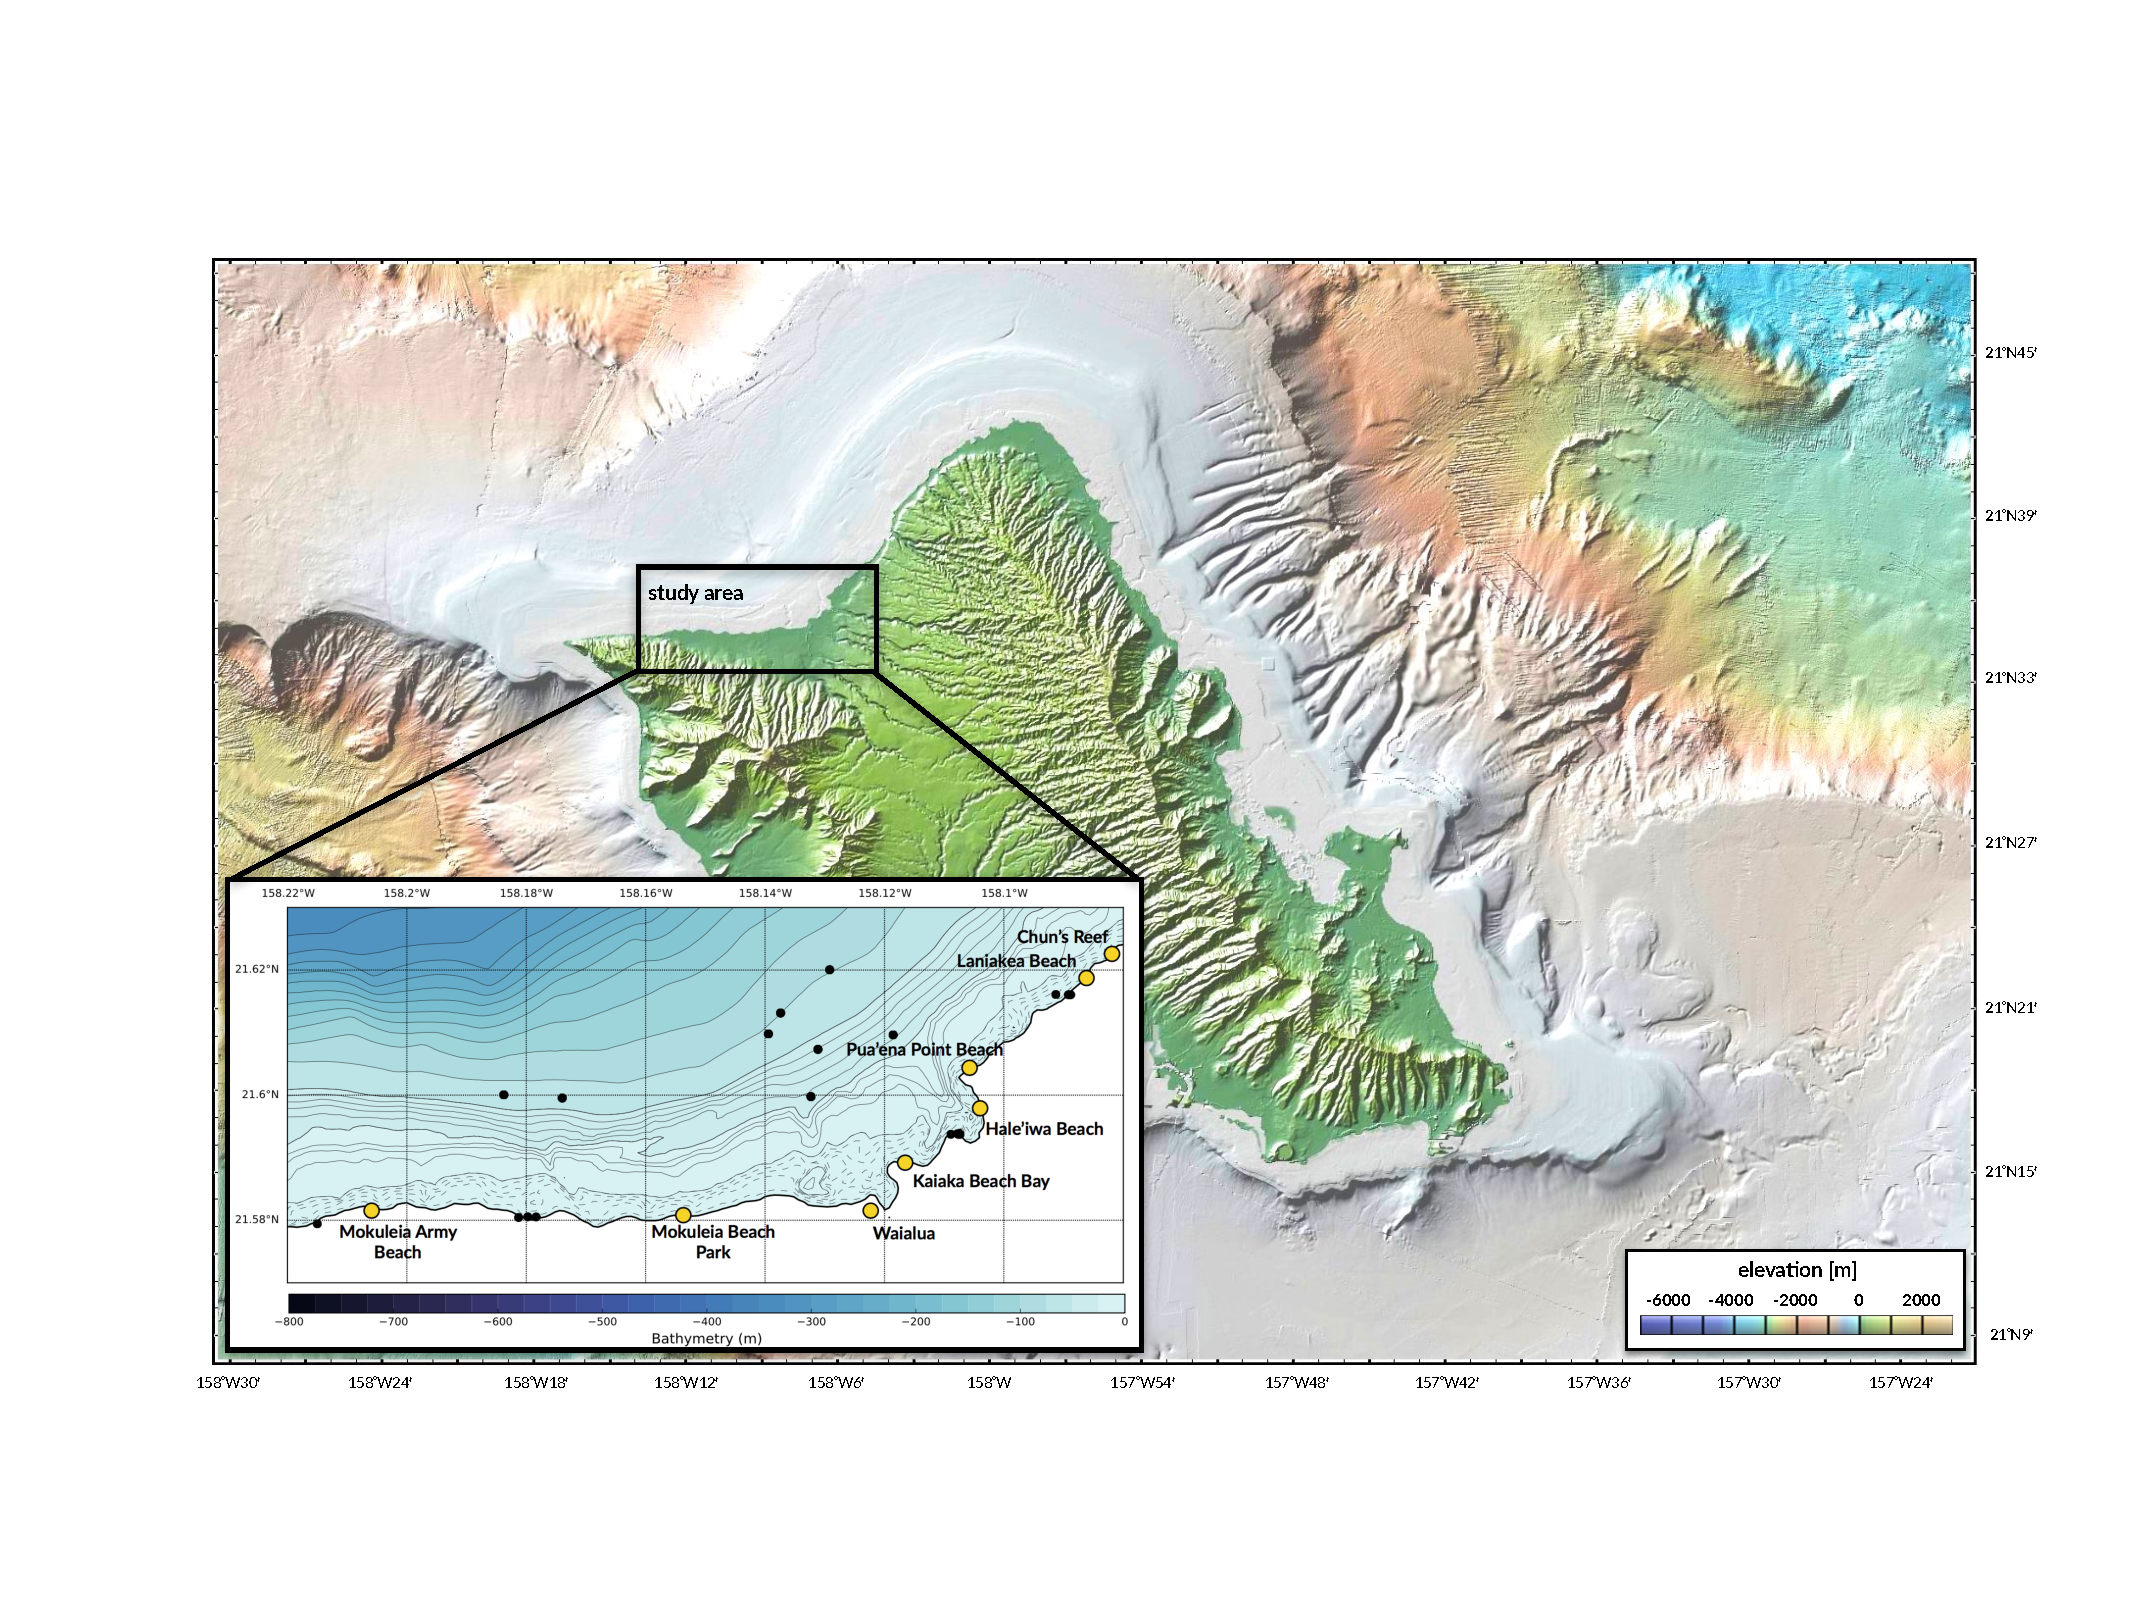
\includegraphics[width=17.8cm]{fig1}
\caption{High-resolution map covering Oahu (Hawai'i) at 1-arc-second resolution developed by the NOAA Center for Tsunami Research. Study area is located on the northwest coast of the island and extent from Mokuleia Army Beach to Chen's Reef from West to East. The bathymetry in the region of interest goes up to 300 m depth on the North but is characterised by a shallow seafloor below 20 m which consists mostly of loose carbonate sands and patchy occurrences of coral and coralline algae growth.}
\label{fig:oahu}
\end{figure*}

\subsection*{Implications for sediment transport}

We propose to evaluate our improved formulation of calcareous sand settling velocity by estimating how it will affect sediment transport. Using North Shore Oahu (Hawai'i) as our study region (Fig. \ref{fig:oahu}), we estimate the Rouse number [Rouse, 1937] for a period spanning from 2011 to 2015 using wave data from the Pacific Islands Ocean Observing System (PacIOOS)[\textbf{ref.}]. The old island of Oahu, especially the North Shore, has many white sand beaches and smoother lava and coral reefs than the rugged lava formations and black sand beaches found on the shore of other Hawai'ian islands [Fletcher et al., 2008]. Using minimum, maximum and mean grain size diameters for the region based on USGS reef-front carbonate sediment deposits dataset [\textbf{ref.}] we derive for both siliciclastic and calcareous sands the different modes of transport: bedload, suspended load and wash load.   

%Fletcher, C. H., Bochicchio, C., Conger, C. L., Engels, M. S., Feirstein, E. J., Frazer, N., ... & Vitousek, S. (2008). Geology of Hawaii reefs. In Coral Reefs of the USA, 435-487. Springer Netherlands.
%Rouse, H. (1937) Modern conceptions of the mechanics or fluid turbulence. Trans. Am. Soc. Civ. Eng., 102, 463? 505.

\begin{figure}%[tbhp]
\centering
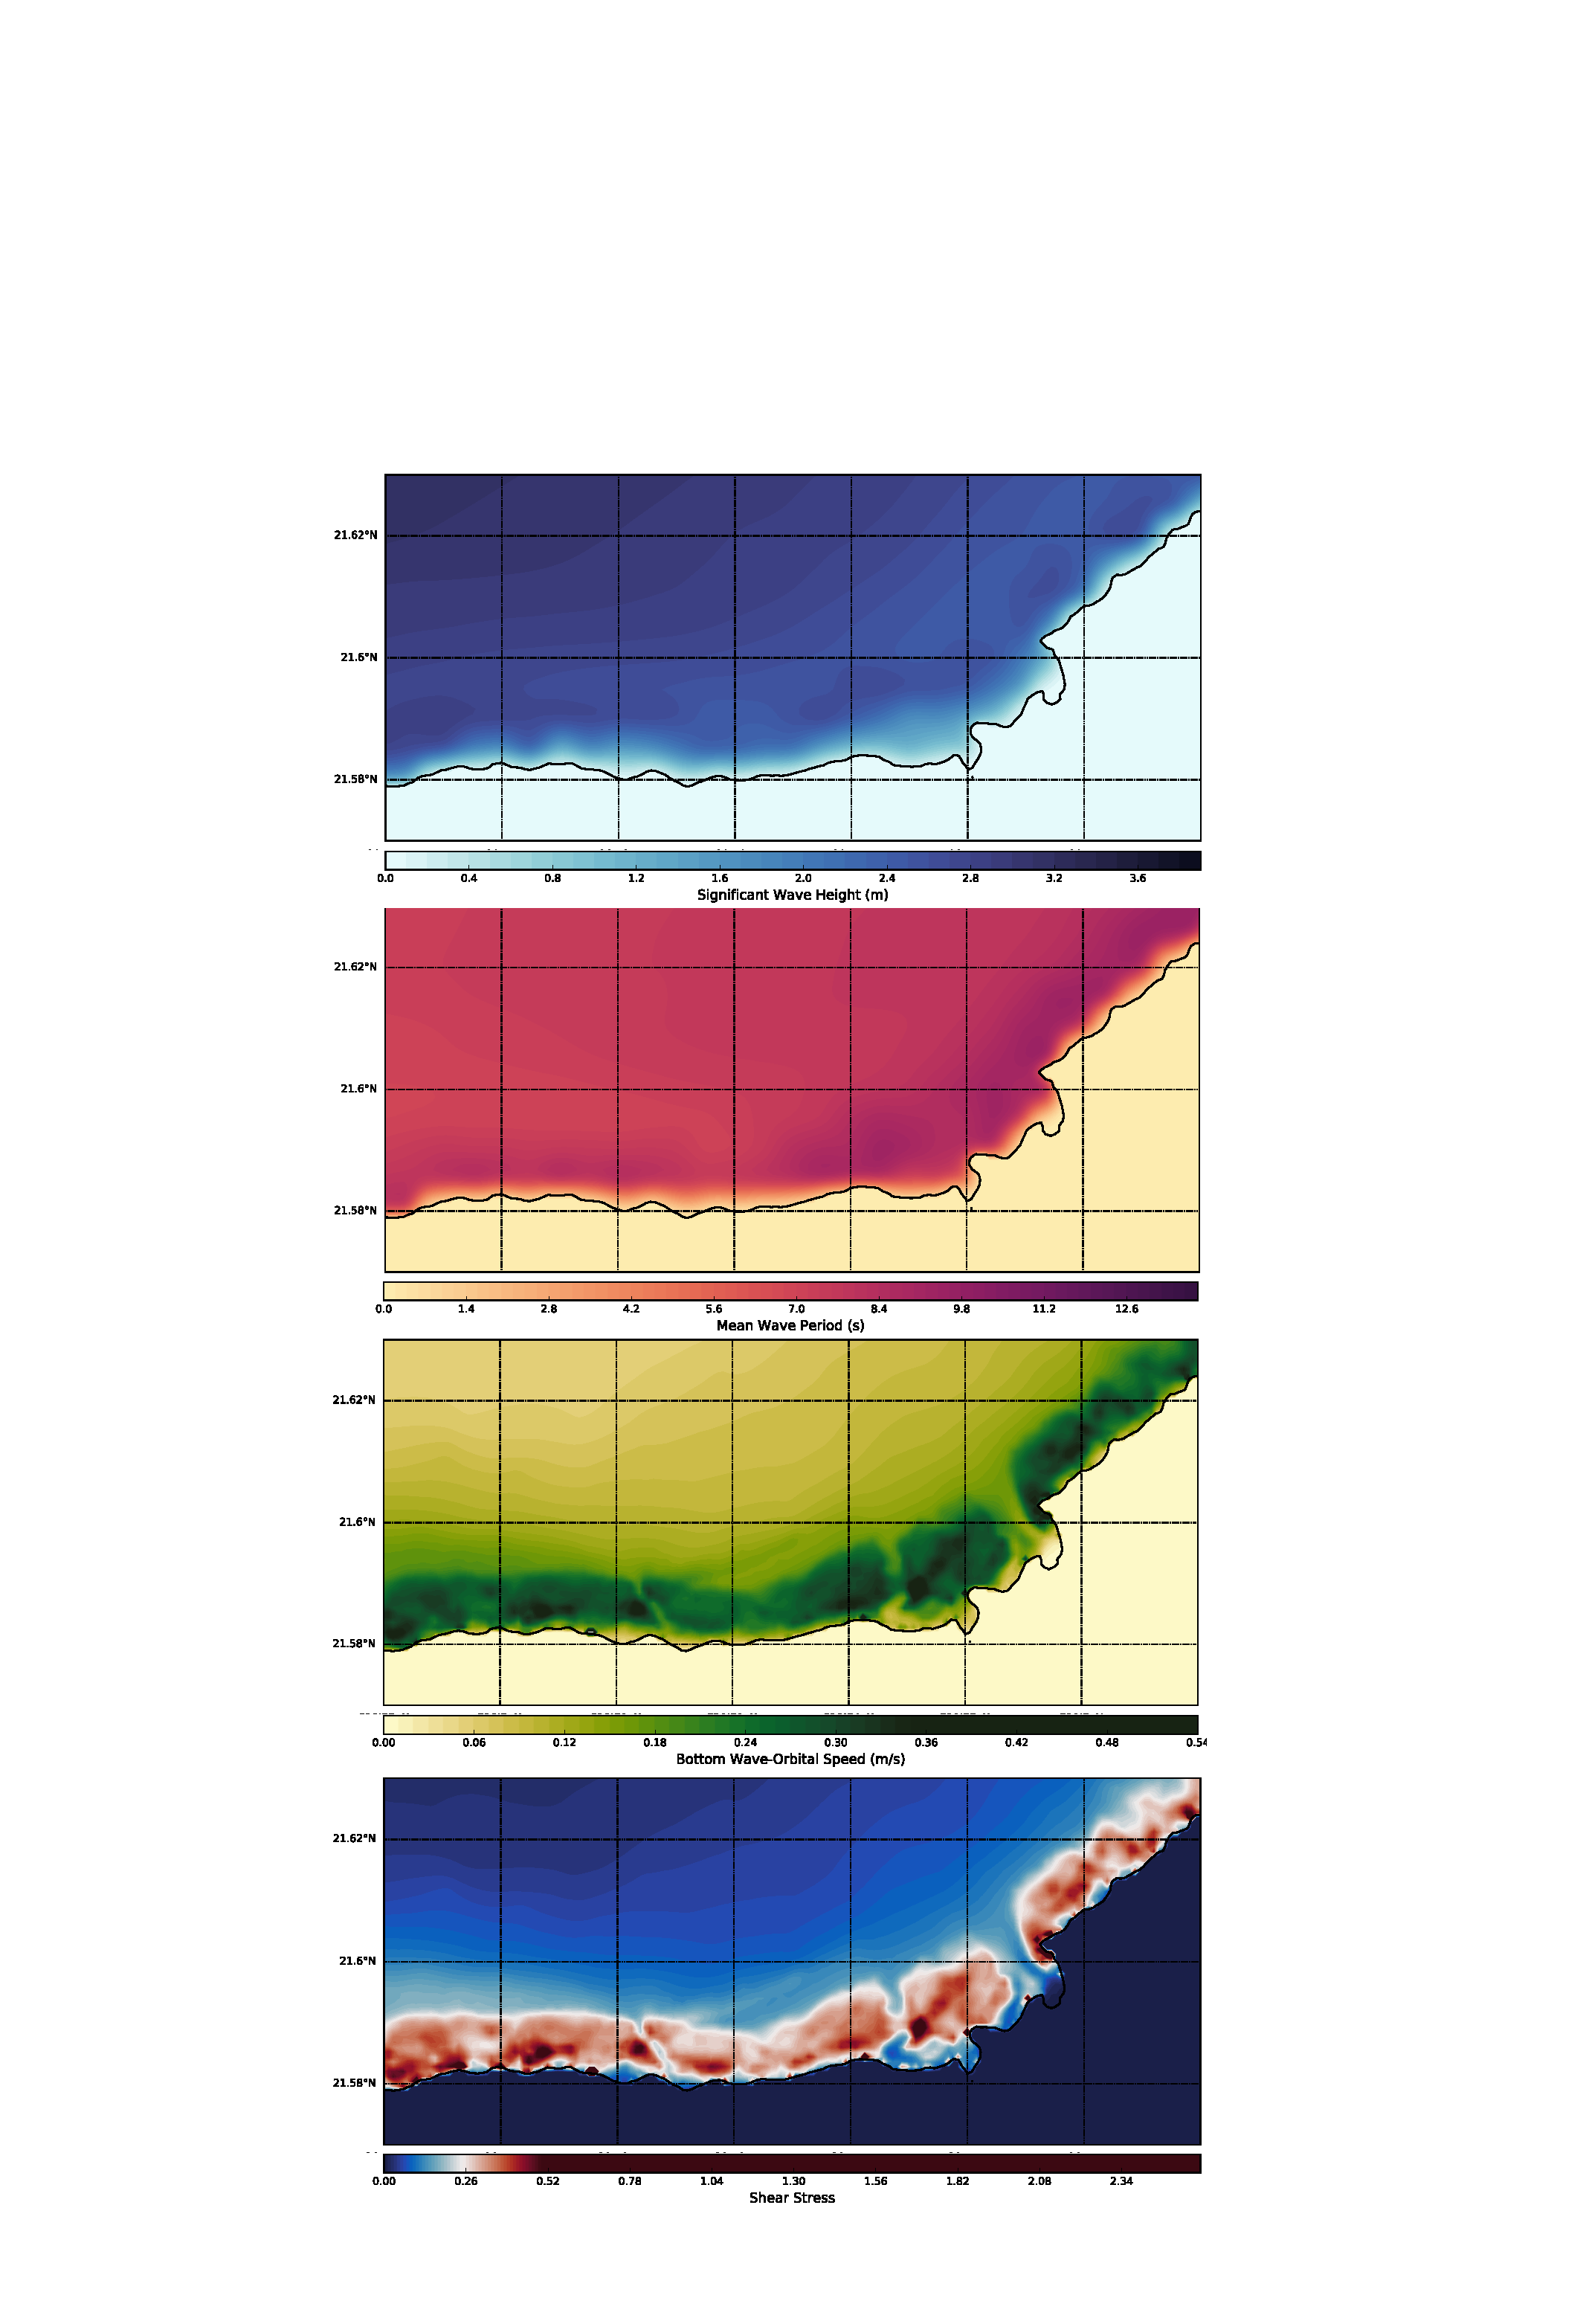
\includegraphics[width=.99\linewidth]{fig2}
\caption{Example of wave-induced bottom shear stress calculated from the PacIOOS SWAN wave dataset for the day 02/03/2013 at 3:00 pm. The two top panels show the significant wave height ($H_s$) and the mean wave period ($T_m$) and are directly extracted from the dataset. The two bottom panels present the horizontal wave-orbital bottom velocity $U_{w,b}$ and the wave-generated bed shear stress $\tau_w$ obtained assuming the linear shallow water approximation and pure wave conditions. }
\label{fig:waveshear}
\end{figure}

\subsubsection*{Wave-induced bottom shear stress}

The wave dataset obtained from PacIOOS is solved with a spectral model SWAN [Booij et al., 1999] and consists of 7-day output with a 5-day hourly forecast at approximately 500 m resolution since June 2010. This high-resolution model is used to capture shallow water effects and nearshore coastal dynamics such as refracting, shoaling, and smaller scale shadowing. Initial boundary conditions for this nested model are obtained from the Hawai'i regional-scale WaveWatch III wave model. From this dataset we extracted for the period ranging from January 2011 to January 2016 the significant wave height ($H_s$) and the mean wave period ($T_m$). \\
Under pure waves (\textit{i.e.} with no superimposed current), the wave-generated bed shear stress $\tau_w$ is typically conceived of as a quadratic bottom friction:
\begin{equation}\label{shear}
\tau_w = \frac{1}{2} \rho f_w U_{w,b}^2
\end{equation}
where $\rho$ is water density, $f_w$ is the wave friction factor, and $U_{w,b}$ is the maximum over-the-wave-cycle horizontal wave-orbital velocity. Inserting into equation [\ref{shear}] the linear shallow-water approximation for $U_{w,b}$, given by:
\begin{equation}\label{uw}
U_{w,b} =(H_s/2)\sqrt{g/h}
\end{equation}
where $g$ is the acceleration due to gravity and $h$ the water depth, yields an expression for $\tau_w$ in terms of the wave height [Green \& Coco, 2013]:
\begin{equation}\label{shear2}
\tau_w = \frac{\rho g f_w}{8} \frac{H_s^2}{h}
\end{equation}
Assuming that the wave boundary layer is hydraulically rough turbulent, the wave friction factor, by definition [Nielsen, 1992], depends solely on the bed roughness $k_b$ relative to the wave-orbital semi excursion at the bed $A_b$. Following Soulsby [1997], we use:
\begin{equation}\label{fw}
f_w = 1.39(A_b/k_b)^{-0.52}
\end{equation}
where $A_b = U_{w,b}T_m$ and $k_b$ is evaluated as a grain roughness [Smith \& McLean, 1977] given as $2\pi d_{50}/12$, where $d_{50}$ is the median grain size of the bed sediment.\\
Most waves in the region reach wave base at approximately 20 m depth and convert their wave energy into shear stress across the sea floor, providing a means for mechanical abrasion of both carbonate framework and direct sediment producers. As an example figure \ref{fig:waveshear} shows the derived values for horizontal wave-orbital velocity and shear stress obtained from PacIOOS dataset.

\subsubsection*{Sediment settling velocities}

In practical applications to bioclastic environments, settling velocities can be used to describe multiple reef zones and to predict sediment transport mode. These applications are critical to understand and predict sediment transport pathways through these systems [Cuttler et al., 2016] but also to evaluate the damage to corals exposed to sedimentation [Rogers, 1990; Weber et al., 2012]. In this study, it is worth noting that we only evaluate the transport of loose sands and therefore do not estimate the impact of reef rugosity on frictional dissipation in the spectral wave model  [Nielsen, 1992; Lowe et al., 2005; Rogers el al., 2015] neither the effect of hard coral disintegration in loose particles.\\
From previous studies on the Oahu shelf, it has been shown that shelf sands are mainly carbonate with only a small percentage of terrigenous content [Moberly et al. 1965; Harney et al. 2000; Harney \& Fletcher 2003]. These calcareous sands accumulate in relatively thin patches, fields, and linear deposits perched on the shallow shelf [Fletcher et al., 2008].  Above the 20 m depth, most sediment on the reef is produced by reef builders, reef dwellers, and reef bioeroders, making this zone the primary source of nearshore sands [Conger, 2005].\\
Information on grain size distribution for the region has been derived from vibracore metadata provided by USGS reef-front carbonate sediment deposits dataset [\textbf{ref.}]. Given the sparse distribution of the dataset and to account for the full extent of calcareous sands grain sizes we perform our Rouse number analysis for three types of nominal diameter (mean, minimum and maximum) set to 0.43, 0.13 and 1.07 mm respectively. \\
The settling velocity for calcareous sands is calculated for each grain size diameter using the drag coefficient ($C_D$) and settling velocity ($w_s$) proposed in equations [xx] and [xx] respectively in which the Corey shape factor ($S_f$) is set to 0.556 [Corey, 1949] and the sediment density ($\rho_s$) to $2600$ kg/m$^3$. Using similar values for $S_f$ and $\rho_s$, the settling velocity for siliciclastic sands is derived from the equations [xx] and [xx] following Riazi \& Turker [2017]. For all diameters, the values of settling velocity for the calcareous formula is below the ones obtained with the siliciclastic approach. 
%Weber M, de Beer D, Lott C, Polerecky L, Kohls K, Abed RMM, Ferdelman TG, Fabricius KE. Mechanisms of damage to corals exposed to sedimentation. Proceedings of the National Academy of Science of the United States of America. 2012;109(24):e699 doi: 10.1073/pnas.1100715109.
%Rogers (1990) Rogers CS. Responses of coral reefs and reef organisms to sedimentation. Marine Ecology Progress Series. 1990;62:185?202. doi: 10.3354/meps062185.
%Cuttler, M. V. W., Lowe, R. J., Falter, J. L. and Buscombe, D. (2016), Estimating the settling velocity of bioclastic sediment using common grain-size analysis techniques. Sedimentology. doi:10.1111/sed.12338

\begin{figure}%[tbhp]
\centering
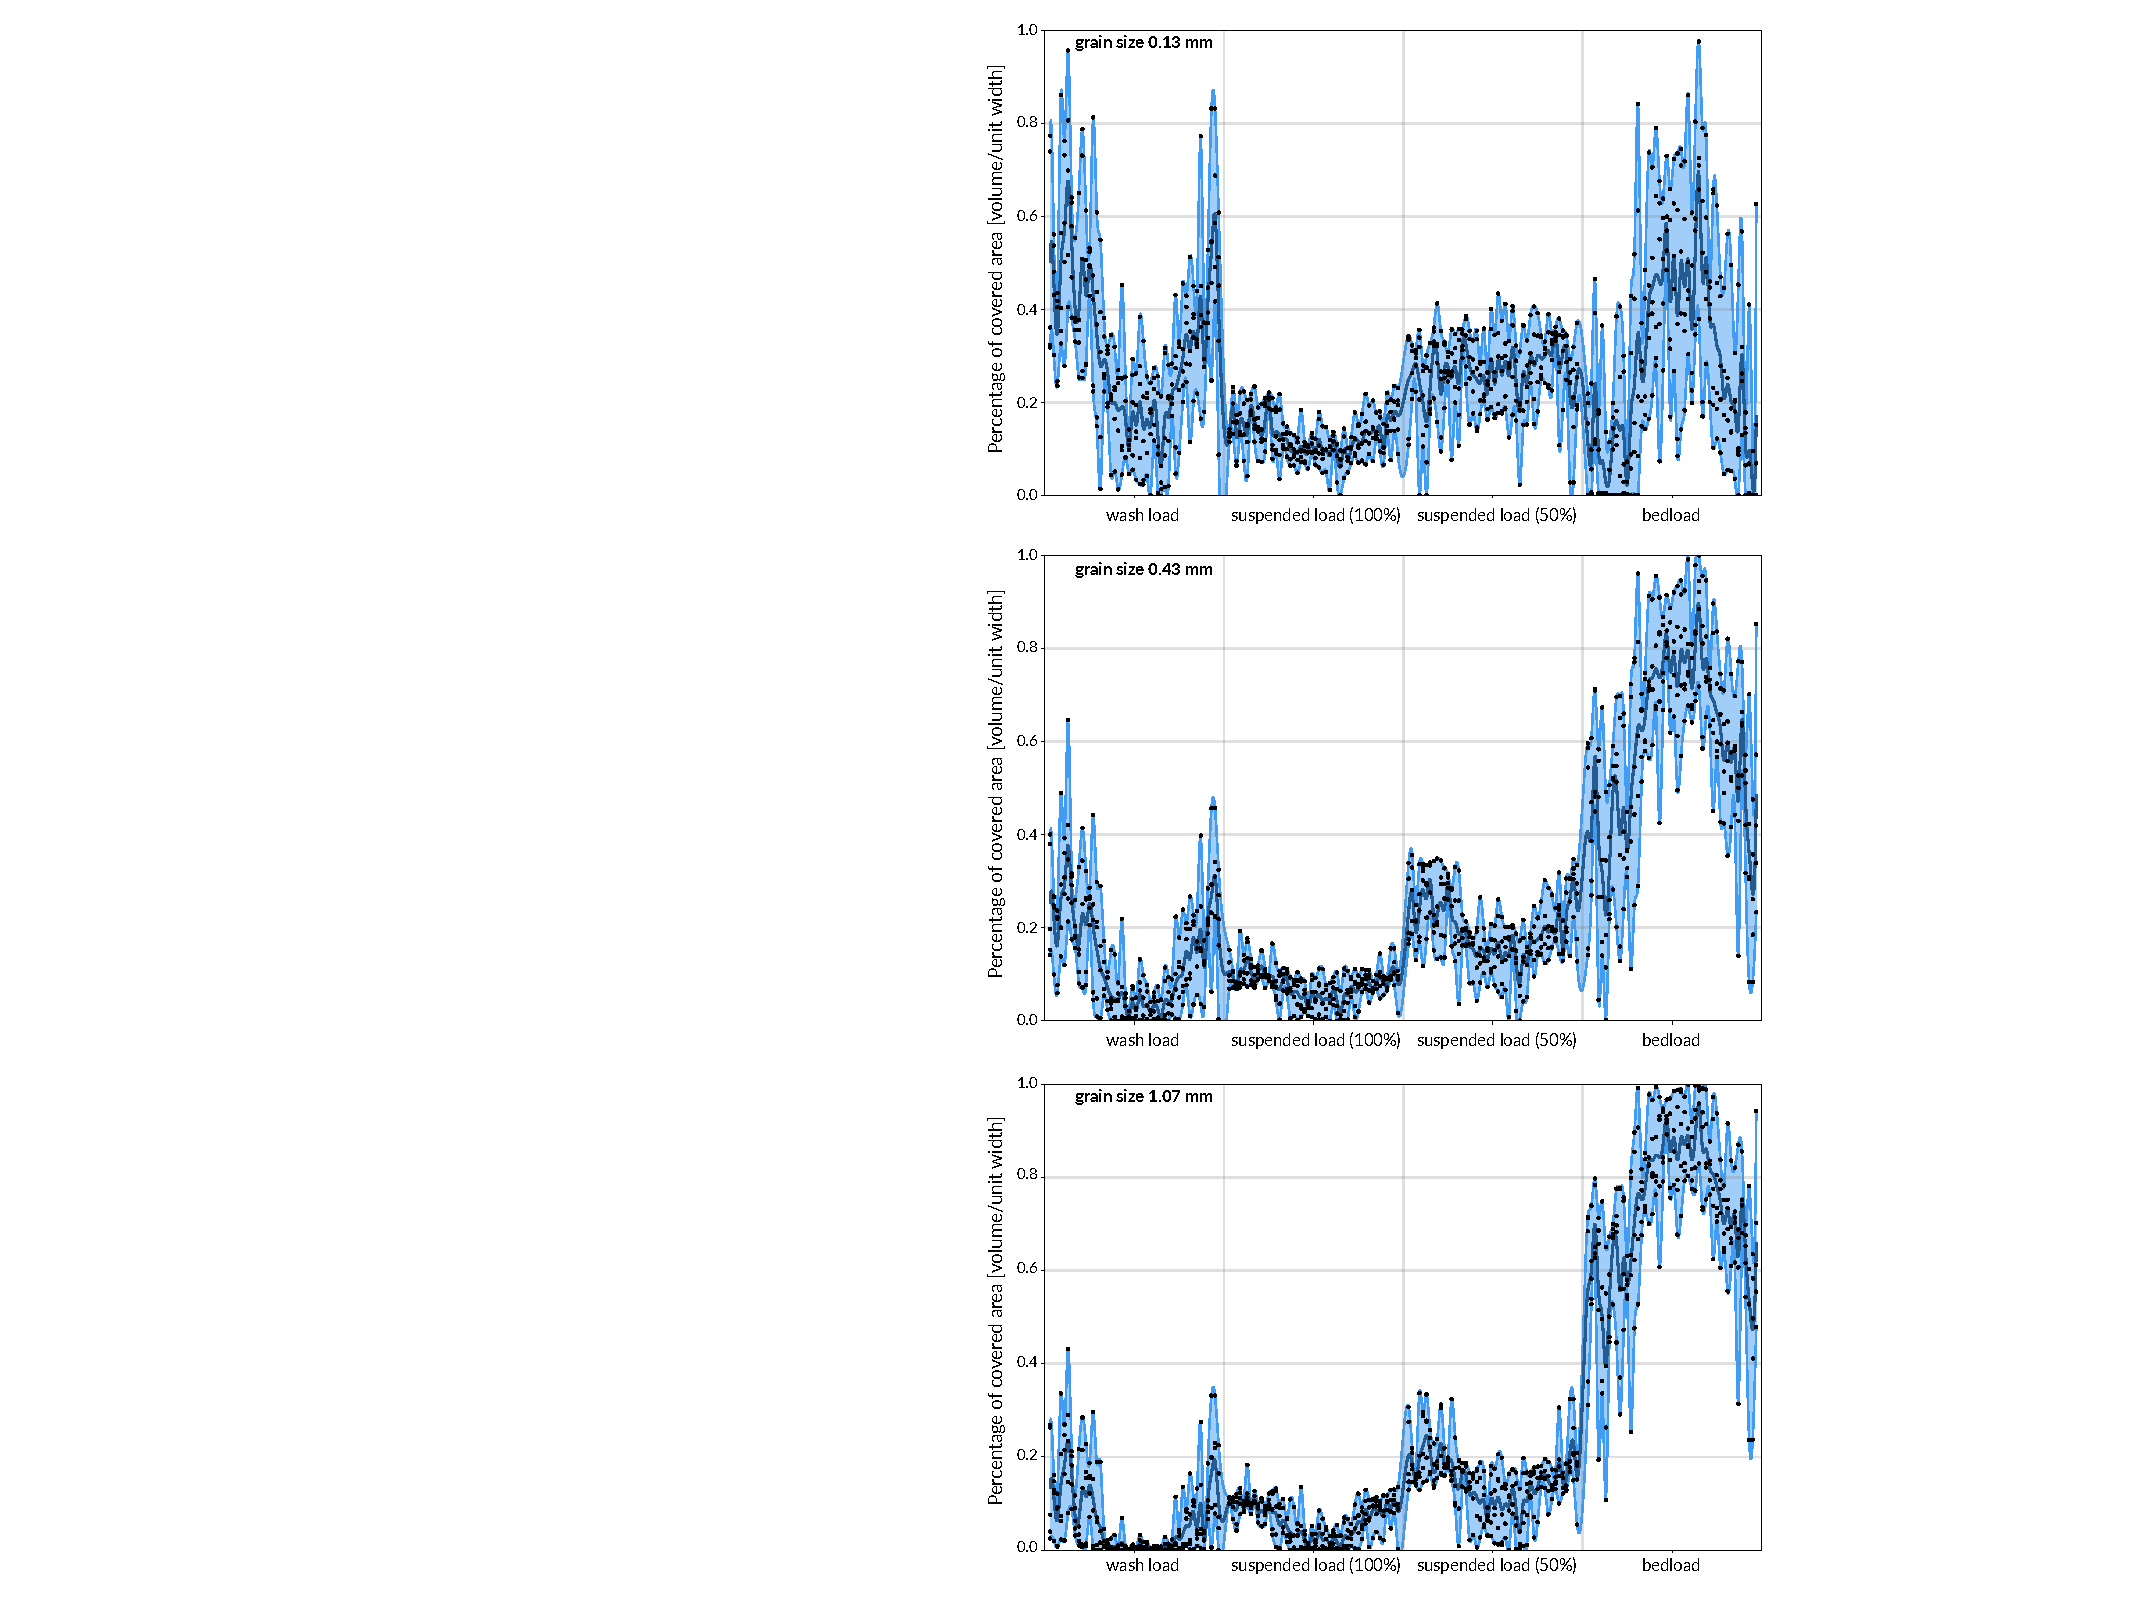
\includegraphics[width=.92\linewidth]{fig3}
\caption{Estimated modes of transport based on our improved formulation of settling velocity for calcareous sands ranging from January 2011 to January 2016. Each panel presents percentage of area covered by 4 types of mode of transport namely wash load, suspended load (50 and 100\%) and bedload over the 5-years of analysed dataset. For each month, three dots representing the minimum, maximum and mean values are plotted. The strong middle line shows the mean of the monthly estimated percentage of area covered and the shaded coloured zone provides the extent (min/max) of the covered area over time. From top to bottom panels, we perform the same analyse with different grain size nominal diameters corresponding to the minimum, mean and maximum values extracted for the studied region from the USGS dataset.}
\label{fig:transport}
\end{figure}

\subsubsection*{Comparisons between calcareous and siliciclastic sands}

As mentioned above, the settling velocity is then used to estimate entrainment and transport mode (bedload, suspended load, or wash load) in the region, using the Rouse number $P$ [Rouse, 1937]: 
\begin{equation}\label{rouse}
P = w_s / (\kappa u_\star)
\end{equation}
where $\kappa$ is the von Karman constant ($0.4$) and $u_\star$ is the shear velocity estimated from the wave-induced bed shear stress $\tau_w$. Sand ripples have been observed in Waimea Bay on the North Shore of Oahu (\textit{ca} 0.15 m amplitude and \textit{ca} 1 m wavelength) [Smith \& Cheung, 2004; Becker et al., 2007] and wave-induced ripple migration (\textit{i.e.} bedload transport) has been suggested to be the primary mode of sediment supply to the shoreline [Fletcher et al., 2008; Cuttler et al., 2015]. \\
Derived settling velocities for siliciclastic and calcareous sands for the 3 grain size diameters are used to calculate $P$ over the 5-years of analysed dataset (Fig. \ref{fig:transport}). The results show that a significant portion of the sediment deposits are mobilised as bedload under the predicted wave conditions enhancing the idea that ripple migration is an important mechanism for shoreline preservation. Typical north shore annual waves have periods of 14-20 s and breaking face heights of 2-15 m. Waves of this magnitude are able to generate and transport a coarse bedload of carbonate gravel. For the minimum grain size diameter (0.13 mm), the estimated Rouse number mainly exhibits 2 modes of transport: wash load and bedload; which fit well with the prevailing major swell directions in the region (\textit{i.e.} North Pacific swell during winter and Southern swell during summer).

%Smith, D. A., and K. F. Cheung (2004), Initiation of motion of calcareous sand, J. Hydraul. Eng., 130(5), 467?472.
%Becker, J. M., Y. L. Firing, J. Aucan, R. Holman, M. Merrifield, and G. Pawlak (2007), Video-based observations of nearshore sand ripples and ripple migration, J. Geophys. Res., 112, C01007, doi:10.1029/2005JC003451.

\begin{figure*}%[tbhp]
\centering
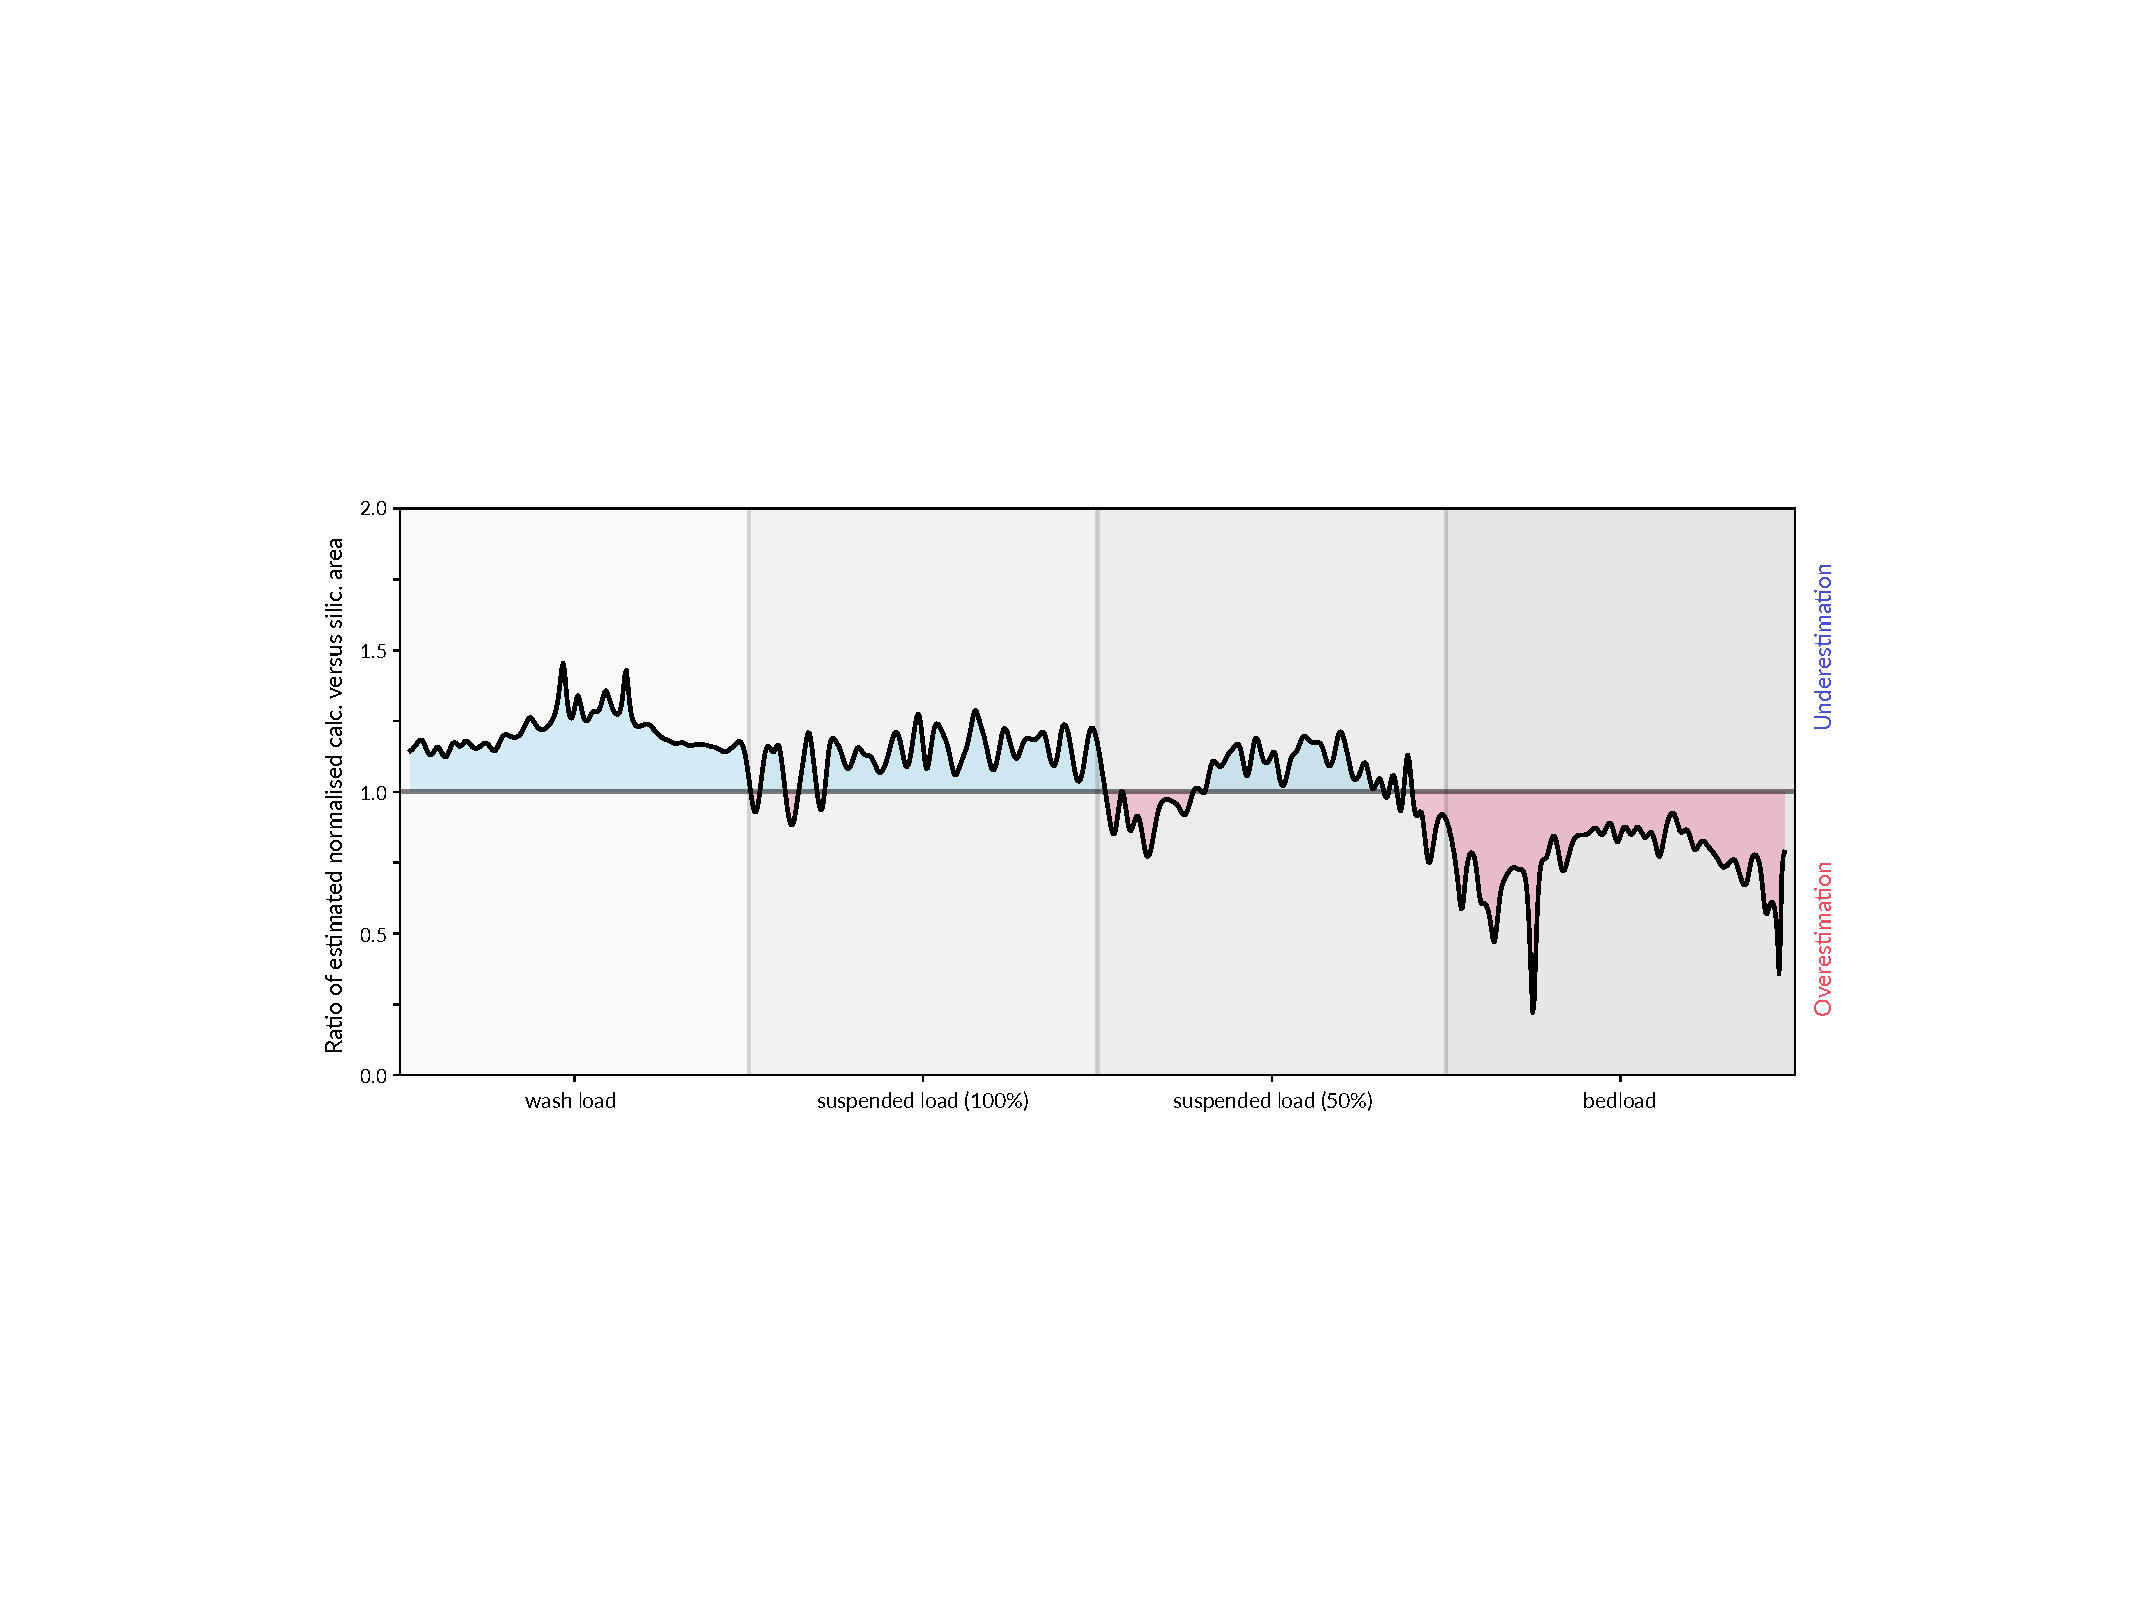
\includegraphics[width=11.4cm]{fig4}
\caption{Comparisons of estimated modes of transport between the two settling velocity formulations for the mean grain size diameters. The ratio between the estimated normalised siliciclastic  versus  calcareous area covered for each mode of transport is plotted. The gray centre line corresponds to the case where both formulations are equivalent. Divergence from this centre line shows either an underestimation of the siliciclastic formulation in respect to the calcareous one when the curve is above 1.0 (blue shaded area) or an overestimation if the curve is below 1.0 (red shaded area).}
\label{fig:diff}
\end{figure*}

Comparisons of estimated modes of transport for the two settling velocity formulations (Fig. \ref{fig:diff}) show that the Rouse number predicted for the siliciclastic sands underestimates both the wash and suspended load modes and over predicts the percentage of bedload transport. This result agrees with the semi-logarithmic plot presented in Figure XX, as calcareous sand settling velocity is always lower than the siliciclastic ones.These differences illustrate the effects of the improved drag coefficient and settling velocity equations on sediment transport modes and could greatly enhance our understanding of sediment dynamics and transport processes in calcareous-rich coastal environments. ... will need additional work...

\end{document}